% Comments --
% 1/11/13 - Proofreading level revision of paper...
%
% 12/10/12 -
%  - incorporate previous work on CRDTs by Preguica, Weiss,  Urso, Molli, Oster, etc.
%
% 03/01/10 - 
%   -Benchmark space complexity of Node extension vs node of size one
%   -Explain the three types of linked lists (section 6)
%   -Work the clash example with the hashtable for node ids, linked list of
%    of global subnodes, linked list of local subnodes.
%   -Create git repository for Dissertation and Collabed.
%   -
% 02/23/10 - Work on the optimization section and lead it into experimental
% results.

% Future work: Intention preserving; Why our approach could really preserve
% a cut and paste (via tree-node transplant) and OPT can't

% 02/17/10 - Starting a new collabed session of the MSET paper.
%     This paper, along with all the images and scripts are
%     stored in a git repository on pythia as "paper-collabed.tex"
%     at address "pythia.cs-i.brandeis.edu/git/mset_paper"

% 7/28 - completed first draft of the paper through the algorithm
%     we still need to add more figures and to revise to make it
%     more readable



\documentclass{amsart}

\usepackage{epsfig}
\usepackage{graphicx}
\usepackage[all]{xy}
\usepackage{pb-diagram}
\usepackage{ulem}

\newtheorem{theorem}{Theorem}[section]
\newtheorem{lemma}[theorem]{Lemma}
\newtheorem{proposition}[theorem]{Proposition}
\newtheorem{corollary}[theorem]{Corollary}



\title{Optimally Efficient Lock-free Collaborative Text Editing}
%
%


\author{
Kenroy~ G.~ Granville
\and 
Timothy J.~Hickey 
}
%\authorrunning{Hickey  and Granville}
%\tocauthor{Timothy J.~Hickey (Brandeis University)
%\and Kenroy~ G.~ Granville (Brandeis University) }
%\institute{Computer Science Department, Brandeis University \\
%\email{\{tim$\mid$kgg\}@cs.brandeis.edu} }

\bibliographystyle{abbrv}

\begin{document}

\maketitle

\begin{abstract}
In this paper we present a new collaborative text editing data type,  
the Monotone Shared Edit Tree (MSET). This algorithm is an extension
and optimization of the TreeDoc datatype of Preguica and Shapiro 
which is one of several new collaborative editing models which are based
on the concept of a Commutative Replicated Data Type (CRDT). 
These models do not rely on locking, are not based on operational transformation,
maintain a local copy of the document with each client,  
and do not require a central server to serialize the edit operations.
Editors based on CRDT allow multiple users to locally 
edit their own copies  of a shared text document
by inserting or deleting characters
while simultaneously sending out local edits 
to remote users and processing edits from remote users 
on their local copy. The primary innovation with MSET is that it
provides an optimally efficient algorithm where 
each edit operation (whether generated locally or remotely) 
requires $O(\log(N))$ time to process, where
N is the total number of characters that have inserted 
into the user's document before the operation in
question is applied (including those characters that were later deleted).
%The MSET algorithm is based on 
%a Model-View-Controller paradigm in which the
%model underlying the text document is a simple and 
%natural type of tree that represents the full collaborative edit process.
%The edits that are allowed for this tree are monotone in the sense that
%the individual edits add a component to the tree which can never be removed
%though it can be evolved in a monotone fashion. For example, deletion is handled by changing the
%visibility attribute of a character from ``visible" to ``hidden''. The tree operations facilitate shared editing as the order in which
%they are applied does not affect the eventual result.
%The key property of the MSET algorithm is that it is convergent, i.e.  
%if all users stop generating
%editing operations, then when all operations have 
%been received and processed, all users will have
%the same document. 
A collaborative editor, CollabEd, 
based on an optimized version of the MSET algorithm 
has been successfully introduced as a plugin into widely used
editors such as JEdit, Eclipse and Netbeans and 
these collaborative editors have been used in classroom situations
with positive feedback from the users (both students and faculty).
\end{abstract}
\newpage
\tableofcontents
\newpage

\section{Introduction}
\label{intro}
Collaborative text editing has a long history stretching back to the dOPT model of Ellis and Gibbs from 1989 \cite{ellis_concurrency_1989}. The dOPT model was the first approach to collaborative editing that didn't require users to "lock" part of the document before begining their edits so as to prevent conflicts between simultaneous editors.

Most of the early work on collaborative editing, beginning with dOPT, used an operational transformation approach with a central server that would serialize all edit operations  and rebroadcast them to the clients \cite{nichols_high-latency_1995}. The server and clients would transform the edit operations they received from each other before applying them to account for differences in the remote documents when the original edit operations were applied. Many extensions and variations of this early work have been developed over the ensuing 25 years (see e.g. \cite{sun_operational_2004}).

In the past few years, a new approach has been developed that greatly simplifies the process of collaborative editing by relying on data types in which the edit operations are commutative and hence do not need to be transformed. These include Uniwiki \cite{oster_building_2010, oster_uniwiki:_2009},  TreeDoc \cite{ letia_consistency_2010, preguica_commutative_2009}, WOOT \cite{oster_data_2006}, LOGOOT \cite{weiss_logoot:_2008, weiss_logoot:_2009, weiss_logoot-undo:_2010}, WOOKI \cite{weiss_wooki:_2007}. These are examples of Commutative Replicated Data Types (CRDT) \cite{preguica_commutative_2009}

Our work, MSET, is a generalization and optimization of the TreeDoc data type  of Preguica, et. al.  \cite{preguica_commutative_2009}. It has been available since 2007 as an open source project hosted at sourceforge \cite{granville_collabed_2007} and has been used as the foundation of the CollabEd system  \cite{granville_collabed:_2009}, which provides a common plugin architecture for code editors allowing developers on different platforms (e.g. jEdit, NetBeans, Eclipse) to simultaneously edit the same code file using the IDE that they individually prefer.

In the rest of this paper we give an overview of the central problems faced by collaborative editors and then we introduce the MSET data type.  The first version is an unoptimized data type which is a simple extension of the TreeDoc model. We then show how to optimize the operations so that every insert or delete operation has time complexity $O(\log(N))$ for the client originally performing the operation and for each client that receives the broadcasted operation, where $N$ is the size number of characters that have been inserted into the document.  In contrast to the approach used in TreeDoc, we do not need to rebalance the tree to obtain optimal performance.



\subsection{The Collision Problem}
The fundamental problem in collaborative editing of any document  
(of any type, not just text)
is dealing with collisions that occur when two 
users (say $A$ and $B$) apply different operators (say $\alpha$ and $\beta$) 
to a shared document. Assuming that both users
start off with the same document $D$, the two users will have two (usually) 
different documents $\alpha(D)$ and $\beta(D)$.
A collaborative editor needs to resolve this conflict, so that both users 
return to the state of having the same document $D'$.
In the Operational Transformation approach, this is done 
by introducing transformed operations $\alpha'=T_\beta(\alpha)$ and 
$\beta'=T_\alpha(\beta)$ as shown in the diagram below,
where $T$ is a transform operator:
\[
\begin{diagram}
\node{D} \arrow{e,t}{\alpha} \arrow{s,l}{\beta} \node{\alpha(D)} \arrow{s,r}{\beta'=T_\alpha(\beta)} \\
\node{\beta(D)} \arrow{e,t}{\alpha'=T_\beta(\alpha)} \node{D'}
\end{diagram}
\]
and the transform operator must be defined so that this diagram commutes, 
that is, there must be an operator $\gamma$ on
$D$ such that:
\[
\alpha'(\beta(D)) = \beta'(\alpha(D)) = \gamma(D) = D'
\]
If this operation holds, we can let $(\alpha \vert \beta)$ denote the combined operation $\gamma$.

If the operators are left invertible then one can define 
the transform operator $T$ in terms of the collision
operator $\gamma$, as follows. Since the operators $\alpha$ 
and $\beta$ are invertible, there must be
operators $\alpha^{-1}$ and $\beta^{-1}$ such that
\[
\alpha^{-1}(\alpha(D)) = D \;\;
\beta^{-1}(\beta(D)) = D 
\]
we then define T as follows:
\[
T_\alpha(\beta) = (\alpha \vert \beta) \circ \alpha^{-1}
\]
Once a collision operator is defined, 
one can implement a collaborative editor which uses a central
server to serialize all of the edit operations into a single stream 
and which applies the transforms to resolve
conflicts among users.  

There are some problems with collaborative editors implemented
using the the Operational Transformation model.  One problem is that the
collision operators need to be implemented in a way that is natural and
intuitive for the users.  Another is that if the latency is high, the time
required to transform individual operations can be unacceptably large.

A final concern is that if the network traffic is temporarily halted and both
clients perform $n$ operations without processing any of the other client's
operations, then the time for them to resync is $O(n^2)$. To see this, let $D_{i,j}$ denote the document obtained by processing $i$ operations from user 1 and $j$ operations from user 2, where both clients start with $D_{0,0}$. If user 1 is at $D_{i,0}$ and user 2 is at $D_{0,j}$, then they will both need to compute $D_{i,j}$ for all $i,j\in[0,n]$ to be able to transform $D_{0,0}$ into $D_{n,n}$. Typically,
user 1 will calculate $D_{i,1}$ for all $i$ from 1 through $n$, then $D_{i,2}$ for all $i$, etc. while user 2 will calculate $D_{1,j}$ for all $j$, then $D_{2,j}$ etc. The MSET algorithm we propose has no added complexity for such network delays and, in fact, we purposely allow the users to enqueue incoming operations (and/or outgoing operations) and this feature would render an Operational Transform system unusable.

\subsection{The Monotone Shared Edit Tree (MSET) approach}
In this paper we present a new algorithm based on a more sophisticated
representation of the string. We call this the 
{\bf Monotone Shared Edit Tree} or MSET representation which is based 
on a model, view, controller paradigm.  The key idea is to use a model for
string editing that maintains three simultaneous views: the usual string editing view, the "revisions" view which shows all of the previously "deleted" code highlighted in someway (e.g. like tracking-changes with strikethrough font), and an "edit-tree" view which gives a more full record of the editing session recording which users made which insertions among other information. Thus, the editing session will be implemented by maintaining a set of models $\{T^u_i: i=0,1,2,\ldots\}$ for each user $u$. These models have several views including the standard view which is the only view in which the user is allowed to edit.  Two local editing operations are allowed: 
\begin{itemize}
\item insert a character $c$ at offset $k$
\item delete the character $c$ at offset $k$
\end{itemize}
Each of these is transformed into an operation $\tau$ on the underlying model and that operation is broadcast to all other users editing the document. Thus,
if we let $S^u_i$ denote the standard view of the string that user $u$ is editing after $i$ edit steps have been applied and if we let $\sigma^u_i$ denote then the
editing operation applied on the string and $\tau^u_i$ denote the corresponding MSET operation, then the following diagram commutes:
\[
\begin{diagram}
\node{T^u_i} \arrow{e,t}{\tau^u_i} \arrow{s,l}{\Gamma} 
\node{T^u_{i+1}} \arrow{s,r}{\Gamma} \\
\node{S^u_i} \arrow{e,t}{\sigma^u_i} \node{S^u_{i+1}}
\end{diagram}
\]
where $\Gamma$ is the projection that converts an MSET model $T$ into the corresponding string view $S=\Gamma(T)$.  When user $u$ performs a local edit $\sigma^u_i$ the system converts that into an operation $\tau^u_i$ on the model, and that operation is applied to the underlying model (thereby changing the standard string view) and is simultaneously broadcast to all peers.  Likewise, when the system receives an MSET transformation from a peer, it places it on a queue and when the user is not editing, it dequeues a transformation $\tau^u_i$ to the model. This corresponds to a string edit operation $\sigma^u_i$ which is what the user sees.  The point is that the MSET system works both ways: transforming local string edits into MSET edits, and transforming remote MSET edits into local string edits. 



The underlying model we use, MSET, has the property that the allowed operations are a naturally partially ordered set  by an editing dependence relationship (e.g. you can't delete a character until you have inserted it, and you can't insert between two characters in a string until you first insert those two characters)
and that any two operations which are independent can be applied in either order with the same result.  If we also assume that the sequence of messages sent from one user to another are received in the same order as they are sent, then this guarantees the convergence property of this collaborative editing scheme, that is when all users stop editing and all messages are delivered, they have the same underlying model $M$ and hence they also have the same edited string.

The MSET algorithm uses peer to peer communication with no central server but it assumes that  the order of messages sent between peers is preserved, and that peers never fail. It allows new clients to join and current clients to leave while preserving convergence. 

\subsection{Structure of the paper}

In section \ref{sec:overview} we provide an overview of the new MSET-based
collaborative editing algorithm by giving an example which clearly illustrates
the underlying model, the transforms, and the three views. The MSET model is a generalization of the TreeDoc data type (although we didn't know about TreeDoc when we first formulated and implemented MSET in 2007 \cite{granville_collabed_2007}). In section \ref{sec:edittrees} we present a simple distributed editing algorithm for edittrees with potentially poor performance (e.g. $O(N)$ time to insert or delete a character)).

The problem with the basic MSET model is that it represents the editing string as a tree which can (and often will) become very unbalanced.  The TreeDoc approach to dealing with this effect is to periodically rebalance the tree by communicating among all of the users (or at least a core group) and temporarily halting the editing while all users agree on a common tree and suspend editing while they converge the document and rebalance the tree.

Our approach is to further enhance the model so that it can still process all local and remote edit operations in time $O(\log(N))$ where $N$ is the size of the tree (i.e. the total number of characters inserted into the tree, even including those that were later deleted). We use the edit-tree to give globally unique names to the positions where a character can be inserted or hidden, but we use a more sophisticated data structure to access and modify the edit tree.
We present this enhanced model, prove its correctness, and bound its complexity
in section \ref{sec:proof}. We then show how it can be used to support optimally efficient collaborative editing in section \ref{sec:collabed} and we discuss some potential problems in section \ref{sec:pitfalls}.


In section \ref{sec:implementation} we discuss our experience with an implementation of MSET that has been used to facility collaboration among users who are simultaneously using different IDES (e.g. Netbeans for user 1, Eclipse for user 2, a homegrown editor for user 3, etc.) and we discuss some of the practical extensions that have proven useful (e.g. queueing incoming and/or outgoing messages, color coding most recent editing changes from various users, etc.). We conclude with some suggestions for future work in this area.

\section{Overview of the MSET algorithm}
\label{sec:overview}

In this paper we propose a method for collaborative editing in which the
users maintain a tree-structured representation of the editing process and
broadcast tree edit operations rather than string-edit operations. The advantage
of this approach is that the tree-edit operations we introduce do not need to be transformed, that is, if they are independent in a sense defined below, then they commute -- $\alpha(\beta(T)) = \beta(\alpha(T))$ and hence can be applied in any order! This greatly increases
the efficiency of the collaborative editing scheme and simplifies the algorithm.


There are several key features of the MSET model, $M$.

\paragraph{\bf simple model}
The underlying tree model is a simple and natural tree representation
of the collaborative edit session. Editing is modeled by allowing users to insert or delete a single character at a specified offset in the string. The system maintains three simultaneous views of the document: $M.S$ the standard string view, $M.R$ the revisions view which also shows the characters that have been deleted (usually with a strike-through font), and $M.E$ the edit tree view in which start and end markers are inserted to fully reflect the structure of the edit tree.

\paragraph{\bf local}
All users transform the string operation into a tree operation
which is performed locally.

\paragraph{\bf peer-to-peer}
The tree operations, once performed locally, are broadcast
to all other users, using a peer-to-peer approach.
Users receive remote tree operations (in any order) though some must
be cached if their target node has not yet been created locally.

\paragraph{\bf convergent} 
When all users stop editing and all messages are delivered and processed, all
users will have the same edit-tree and hence the same string
views.

\paragraph{\bf optimally efficient}
Each local insertion and deletion operation takes time $O(\log(N))$ where $N$ is the size of the edit-string, and each remote insertion or deletion operation received from peers also takes at most $O(\log(N))$  time to complete, assuming that its target has been received.  If the target has not been received, it is cached until it can be applied. This delay is not counted in the $O(\log(N))$ time bound.

\paragraph{\bf generalizable}
The model can be generalized so that each character can have attributes
from any attribute set (font, style, color, etc.) and any user can change the
attributes at any time. The properties above 
all remain for this more general model, except that the model is slightly
more complex.

\paragraph{\bf practical} 
This model has been used to create collaboration plugins for several
popular editors and IDEs including JEdit, Eclipse and NetBeans. These
collaboratized editors have been used in Computer Science classes
and have been found easy and natural to use by students and faculty
alike.

\subsection{Comparion to Operational Transformation}
The collaborative editing algorithms based on Operational Transformation generally satisfy the three properties listed below.
As we explain, MSET satisfies the first, doesn't satisfy the second, and may or may not satisfy the third depending on whether
cut/paste operations are allowed as atomic operations.
\begin{enumerate}
\item {\bf convergence property} - after all editing has ceased and the system has become quiescent then all users will
have exactly the same document.  We will prove that the MSET algorithm is convergent. 
\item {\bf causality preservation} - if a given user performs operation A before operation B, then for all other users
the transformed operation A is performed before the transform of the operation B.  The MSET algorithm 
{\it is not causality preserving}. 
For example, if user $u_1$ inserts several
substrings into an initial string $\alpha$, then the algorithm will not necessarily preserve the order in which those operations
were performed when they are sent to the other members of the collaborative editing group. Indeed, user $u_1$ may insert a character $c$ into a word $w$ created by user $u$ and then insert $c'$ into a word $w'$ created by user $u'$.  If user $u'$ receives $w$ after it receives $c$ and $c'$, then it will delay $c$ and insert $c'$ first.  This is a clear violation of causality in a strict sense.  On the other hand, we define a more restricted notion of dependence of operations, and MSET does respect that partial order which is a kind of causality preservation.
\item {\bf intention preservation} - if a given user performed an operation A on a document, then the transform of that operation
should have the same ``intention'' when it is performed in all other user's documents. 
The MSET algorithm is intention preserving in an editing regime that only allows insertion and
deletion, but it is not intention preserving if one also allows cut/paste as an atomic operation. More precisely, if user A is working
on a section of a document and user B cuts away a substring containing A's work and then pastes that section into another part
of the document. One might expect that A's position in the string would be moved to the new part of the string and although 
A might find this transport disorienting, at least there would be no break in the continuity of ``A's'' editing.  
This is not what happens with MSET.
Indeed, User A would suddenly find the text around his/her position deleted and, if there was some latency, 
the characters A had been typing would appear in this deleted region. User A will then have to search for the moved text.
\end{enumerate}


\subsection{A simple example of the MSET algorithm}
Let us assume that we have several users $u_0,u_1,\ldots$ who are
collaboratively editing a shared document. Each user $u$ maintains a local
copy $S^u_i$ of the string being edited and also maintains a more complex representation of the editing process
which we will call an edit-tree.
This edit-tree $T^u_i$ represents the string and all edits that have been
performed on it. There is a natural projection $\Gamma$ from edit-trees to
strings such that $\Gamma(T_i)=S_i$ and this invariant will be maintained.
The users can also switch to a "revision-string" view $\Gamma_R(T^u_i)=R_i$ which
shows the deleted characters also, or an "edit-string" view $\Gamma_E(T^u_i)=E_i$
which shows a string representation of the tree using start and end markers for each node.  The examples below will
make this clear.

\subsubsection{Initial state}
All users start out with the empty string $S^u_i=""$ where the
tree representation $T^u_i$ is a single node owned by user $u_0$, the superuser,
and containing only the start and end marker symbols $<^0_0$ and $>^0_0$ for the 0th node of user 0. These markers appear only in 
 the edit-string view.
\begin{align*}
E^u_0 &=& <_0^0 \;\;\;\;\;\; >_0^0 \\
R^u_0 &=& \epsilon\\
S^u_0 &=& \epsilon
\end{align*}
where $\epsilon$ denotes the empty string.
MSET only allows users to edit the standard view, $S^u_i$, of their document. They may insert or delete characters anywhere in $S^u_i$, but the other two views are purely read-only.

Each node in the edit-tree is owned by
a single user $u$ and the nodes owned by a user $u$ also have an index $n$
which uniquely identifies them for that user. 
Thus each node
is uniquely identified by the pair $u/n$ of user id and node index.
The index $n$ is the number of nodes that have been created by $u$ before
the current node so it doesn't depend on how many nodes any other user
has created. It is a purely local counter for user $u$.

The user $u_0$ represents the
system and owns only one node, the root. User $u_0$ also does no editing on
the document.

\subsubsection{Inserting a string}

If user 1 inserts the sentence ``This is an example.'' 
the string operation on $S_1$ is
\begin{verbatim}
  stringinsert(0,"This is an example")
\end{verbatim}
which is translated into the following edit-tree operation
\begin{verbatim}
  treeinsert(u0/n0,0,u1/n0,"This is an example")
\end{verbatim}
which states that a new node, $u1/n0$, should be inserted as a child of
node $u0/n0$ at position $p=0$. This operation is then broadcast to all of the
peers who apply it to their own trees $T_j$.
The corresponding edit-tree is shown in Figure \ref{fig:tree0} and the
corresponding string views become 
\begin{align*}
E^{u_1}_1 &=& <_0^0 <_0^1 \text{This  is  an  example.}>_0^1 >_0^0\\
R^{u_1}_1 &=& \text{This  is  an  example.}\\
S^{u_1}_1 &=& \text{This  is  an  example.}
\end{align*}
In practice, user 1 would insert the sentence one character at a time
and the node would be constructed incrementally.
After inserting the first character ``T'' the node $(u1/n0:1)$ would be created
containing only the letter ``T''. After inserting the next character, ``h'',
the system would generate an {\tt extend} operation which would add the
next letter to the end of the node. This is only possibly if the user making
the extension is the owner of the node and if the new character is inserted
at the end of the node.



\begin{figure}[h]
\centering
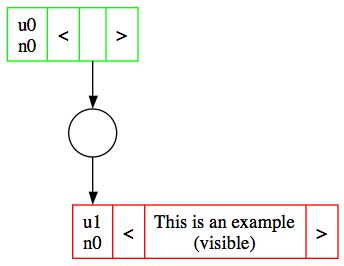
\includegraphics[width=2.0in]{tree1zz.jpg}
\caption{Tree after inserting "This is an example.\label{fig:tree0}"}
\end{figure}

\subsubsection{Inserting a substring}
Next suppose that the user 1 decided to insert the word "interesting"
before "example."  This can not be handled as an extension of the node
$u1/n0$.  As above, this will actually be inserted one character at a time
in most cases (unless the user cut and pastes the word from some other
document into the buffer). Since this is an insertion in the middle of a node,
the system will generate a tree-edit operation which adds a new node $u1/n1$
containing the character $i$ and attaches that node at position 11 of the
parent node $u1/n0$.  As the user continues to type the word "interesting"
the successive characters are added to the node $u1/n1$ as $u1$ is the owner
of the node and the insertions are at the end of the node. The result
is a new node containing the entire word "interesting" attached at position
11 of its parent. The tree in the left side of Figure \ref{fig:tree11}
shows the resulting edit-tree.



\subsection{Creating conflicts in collaborative editing}
Next, suppose user $u3$ 
simultaneously inserts the adjective "illustrative "
before the word "example" in her own
local copy and that both users $u1$ and $u3$ broadcast their edits to their peers, which
includes user $u2$ who is just watching the other two edit.  
In a high latency environment (or in a setting where the users are queueing 
their edits before sending them out), user $u2$ would create its own tree
but with a different node attached at position 11 of the $u1/n0$. This tree
is shown in the right side of Figure \ref{fig:tree11}. Again, if user $u3$
is typing the word character by character then the first character will generate
the node $u3/n0$ containing only one character.

Lets look at this more closely.
We assume at a given point in time all users share the same edit-tree as shown 
in Figure \ref{fig:tree0}. Then they all have the string view
\[
S^u_i= \text{"This is an example."}
\]
Now, if user 1 applies the string operation
\begin{verbatim}
  insert(11,"interesting ")
\end{verbatim}
this will be translated into the following edit-tree operation
\begin{verbatim}
  treeinsert(u1/n0:19,11,u1/n1,"interesting ")
\end{verbatim}
which states that the new node $u1/n1$ containing the text "interesting"
should be added as a child of the node $u1/n0$ at position 11 out of 19. Applying
this operation results in the edit-tree in the left side of Figure \ref{fig:tree11}
and in the following edit-string view
\[
 <_0^0 <^1_0 
 \text{This is an }<^1_1 
 \text{interesting}
>^1_1  \text{example.} >^1_0 >_0^0
\]
Similarly for user 3 who applies the string operation
\begin{verbatim}
  insert(11,"illustrative ")
\end{verbatim}
which is translated into the following edit-tree operation
\begin{verbatim}
  treeinsert(u1/n0:19,11,u3/n0,"illustrative ")
\end{verbatim}
resulting in the following edit-string corresponding to the edit-tree
in the right side of Fig \ref{fig:tree11}
\[
 <_0^0 <_0^1 
 \text{This is an} <^3_0 
 \text{illustrative}
>^3_0  \text{example.} >_0^1 >_0^0
\]


\begin{figure}[h]
\vspace{\baselineskip}
  \hspace{\fill}\rule{\linewidth}{.7pt}\hspace{\fill}
  \vspace{\baselineskip}

\centering
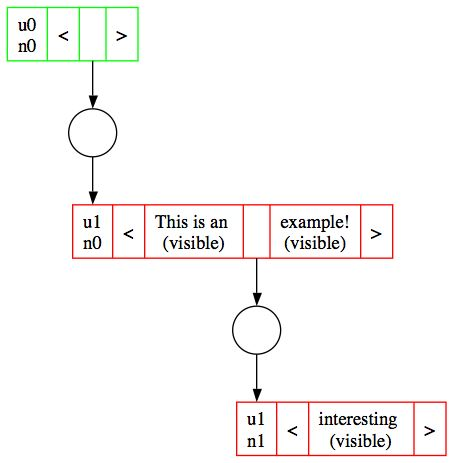
\includegraphics[width=2in]{tree11.jpg}
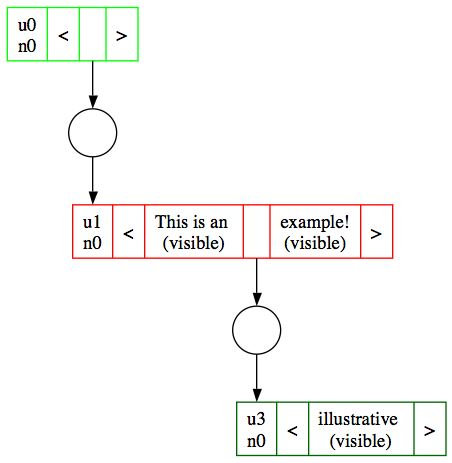
\includegraphics[width=2in]{tree12.jpg}
\caption{Tree $T_1$ on the left after user 1 inserts "interesting ,
and tree $T_3$ on the right after user 3 inserts "illustrative ".\label{fig:tree11}}

\centering
\vskip 0.3in
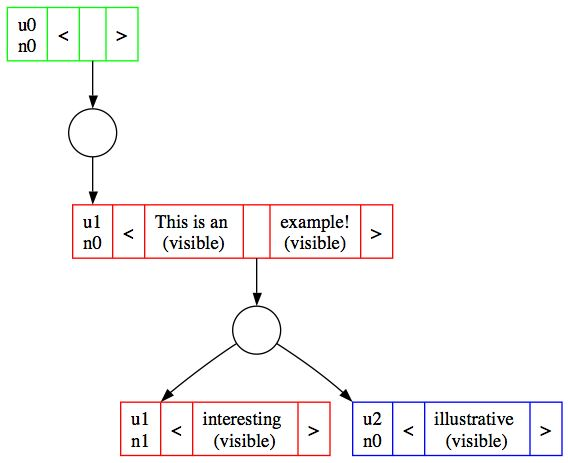
\includegraphics[width=3in]{tree13.jpg}
\caption{Trees after inserting both "interesting " and "illustrative ".\label{fig:tree13}}


\vspace{\baselineskip}%
  \hspace{\fill}\rule{\linewidth}{.7pt}\hspace{\fill}%
\vspace{\baselineskip}%
\end{figure}

\subsection{Handling conflicts in collaborative editing}
When user $u_2$ receives these tree-edit operations there will be an
apparent conflict. Both $u1$ and $u2$ want to insert a string at position
$11$ of $u1/n0$.  

The MSET approach is to allow multiple users to insert at
the same position, but to order the insertions by user id, and to disallow
the same user from inserting multiple times at the same position in the edit-tree.
Thus, if there are $k$ users, then there could be up to $k$ children nodes
attached at any particular position of an edit-tree node.

In this case, conflict resolution results in the tree in Figure
\ref{fig:tree13} where $u1/n0$ has two children nodes attached at position $11$,
the node $u1/n1$ is on the left and $u3/n0$ on the right as $u1<u3$.
This strategy for handling conflicts guarantees that all users will have
the same edit tree, no matter which order they apply the edit-tree operations.

In the case where the new nodes were created one character at a time, rather
than using cut/paste to insert the words, the conflict would occur with two
nodes that each contain a single character and will be resolved in the same
way.  Also, the users doing the editing, $u1$ and $u3$, will receive a
conflicting edit operation and will create the correspond nodes and modify
their string views without changing the relative cursor position. Thus as they
continue typing their edits will be used to extend their nodes and the
same tree will result as if they had used cut/paste to insert the words.


\subsection{Deletion as hiding}

We handle deletion by marking characters stored in the nodes of the edit-tree 
to be either "visible" or "hidden."  Deleting a substring in the standard string
view of the document is translated into an edit-tree operation where the
corresponding characters are marked as "hidden."  Any user can "hide" any
characters, even in nodes they do not own, but no user can "unhide" characters.
Once they are deleted they cannot be made visible again. Rather one must
reinsert the characters.


Continuing with our example, supposer user 1 receives user 3's edits
and so has the string view
\[
\text{This is an interesting illustrative example.}
\]
and deletes the word "interesting". 
The deletion gets transformed into a "hide" operation which results in the
tree in Figure \ref{fig:tree14} which has the following string views:

\begin{align*}
E^{u_1} &=& 
 <^0_0 <^1_0 
 \text{This is an } 
   <^1_1 \text{\sout{interesting }} >^1_1
  <^3_0 \text{illustrative } >^3_0
  \text{example.} >^1_0 >^0_0\\
R^{u_1} &=& 
 \text{This is an } 
    \text{\sout{interesting }} 
   \text{illustrative } 
  \text{example.} \\
S^{u_1} &=&  
\text{This is an } 
   \text{illustrative } 
  \text{example.}
\end{align*}


\begin{figure}[h]
\vspace{\baselineskip}
  \hspace{\fill}\rule{\linewidth}{.7pt}\hspace{\fill}
  \vspace{\baselineskip}
\centering
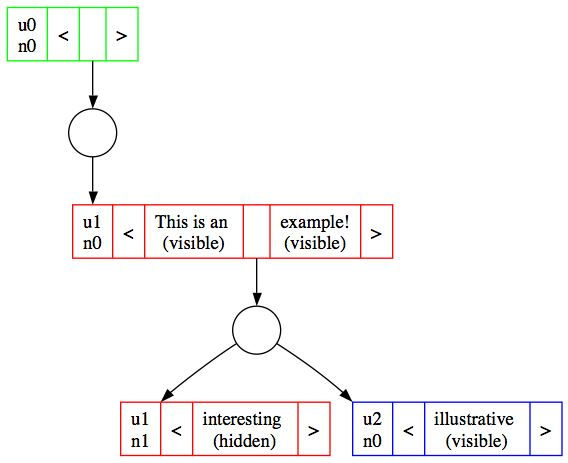
\includegraphics[width=2in]{tree14.jpg}
\caption{Deletion as hiding. Observe that the node $u1/n1$ has the
label "hidden"  beneath its text, whereas the other nodes have "visible".
This indicates that all text in that node is "hidden". \label{fig:tree14}}

\vspace{\baselineskip}%
  \hspace{\fill}\rule{\linewidth}{.7pt}\hspace{\fill}%
\vspace{\baselineskip}%
\end{figure}


\subsection{Inserting into a tree with hidden characters}
Suppose now that user 2 has received all of these edits
and wishes to insert the word ``easy''
into the place where ``interested'' had just been deleted by user 1.
This would result in the following string:
\[
\text{This is an easy illustrative example.}
\]
The point we want to make here is that there are several places that the new node
$X = <^2_0 \text{easy} >^2_0$ could be inserted in the tree
which would place it between "an" and "illustrative" in the string view.
Several possibilities are shown below and their corresponding edit-trees
are snown in Figures \ref{fig:tree14a} and \ref{fig:tree14b}:
\begin{itemize}
\item {\bf leftmost insertion}
The first possibility is to insert the new node directly before the
first character (visible or hidden) after the insertion point. This
is in fact what the current implementation of MSET would select
for this particular example,
but any of these operations could be used.
\[
 <^0_0 <^1_0 
 \text{This is an} 
   <^1_1 <^2_0 \text{easy} >^2_0 \text{\sout{interesting}} >^1_1
  <^3_0 \text{illustrative} >^3_0
  \text{example.} >^1_0 >^0_0
\]
\item {\bf rightmost insertion}
The next is to insert it as far to the right as possible in
the edit-tree.
\[
 <^0_0 \;<^1_0 
 \text{This is an} 
   \;<^1_1 \text{\sout{interesting}} >^1_1\;
  <^3_0 \;<^2_0 \text{easy} >^2_0 \;\text{illustrative} >^3_0\;
  \text{example.} >^1_0\; >^0_0
\]
\item {\bf insertion in a hidden string}
Yet another possibility is to insert it somewhere else (anywhere) in the node $u1/n1$
which contains only hidden text.
\[
 <^0_0 <^1_0 
 \text{This is an} 
   <^1_1 \text{\sout{interesting}} <^2_0 \text{easy} >^2_0>^1_1
  <^3_0 \text{illustrative} >^3_0
  \text{example.} >^1_0 >^0_0
\]
\item {\bf insertion as a child of $u1/n0$}
The final possibility is to insert it as another node at the same level
as $u1/n1$ and $u3/n0$, which only works because coincidentally $u2<u3$. This  would result in
\[
 <^0_0 <^1_0 
 \text{This is an} 
   <^1_1 \text{\sout{interesting}}>^1_1
   <^2_0 \text{easy} >^2_0
   <^3_0 \text{illustrative} >^3_0
 \text{example.} >^1_0 >^0_0
\]
\end{itemize}
These are all the possible ways in which the edit observed in the string view
could be obtained by a valid edit on the edit-tree.

\subsection{Insertion points depend on the user}
Note, the set of such possible edits depends on which user was doing the
editing. Indeed, 
if the word "easy" had been inserted by user 1 instead of user 2,
then another possiblility
would arise. 

{\bf extension of a hidden node owned by the user}
User 1 could just extend the node $u1/n1$
and not create a new node at all, as shown below and in Figure \ref{fig:tree14d}.
\[
 <^0_0 <^1_0 
 \text{This is an} 
   <^1_1 \text{\sout{interesting}easy}>^1_1
  <^3_0 \text{illustrative} >^3_0
  \text{example.} >^1_0 >^0_0
\]


\begin{figure}[h]
\vspace{\baselineskip}
  \hspace{\fill}\rule{\linewidth}{.7pt}\hspace{\fill}
  \vspace{\baselineskip}

\centering
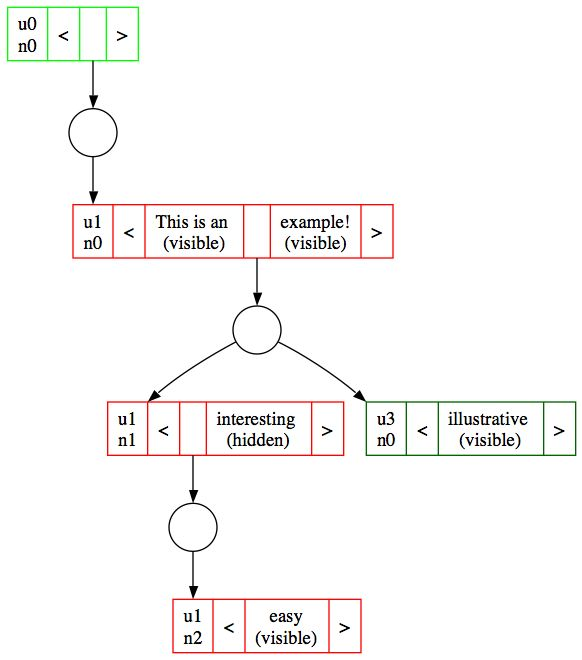
\includegraphics[width=2in]{tree14b.jpg}
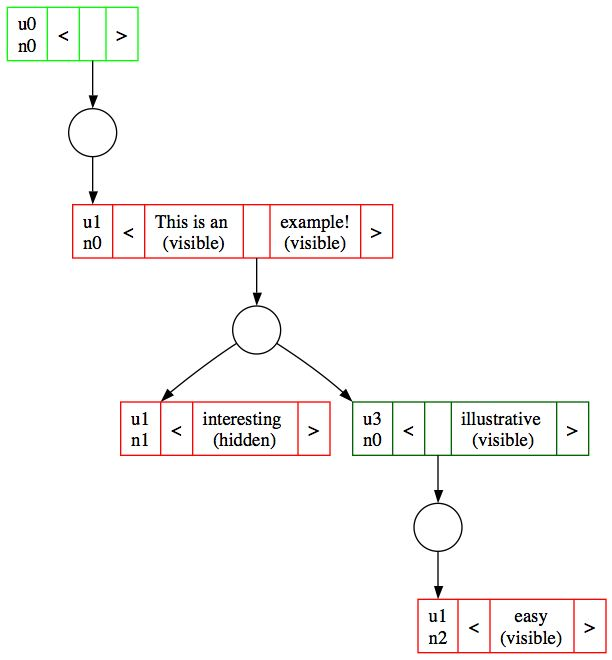
\includegraphics[width=2in]{tree14a.jpg}
\caption{Two ways for user 1 to insert ``easy '' 
between ``an '' and ``illustrative ''. The MSET algorithm
would generate the tree on the left. \label{fig:tree14a}}

\vspace{\baselineskip}%
  \hspace{\fill}\rule{\linewidth}{.7pt}\hspace{\fill}%
\vspace{\baselineskip}%
\end{figure}


\begin{figure}[h]


\centering
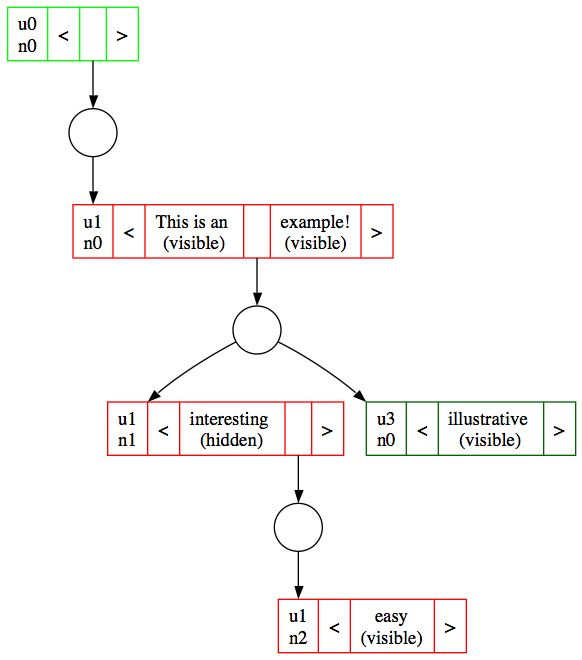
\includegraphics[width=2in]{tree14c.jpg}
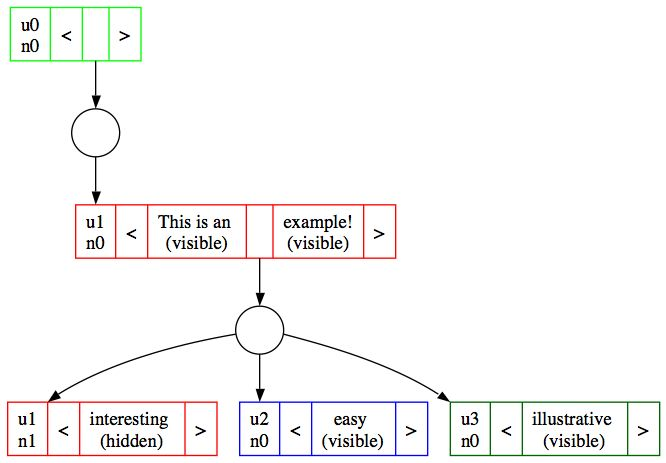
\includegraphics[width=2in]{tree14e.jpg}

\caption{Two more ways for a user to insert ``easy '' 
between ``an '' and ``illustrative ''.\label{fig:tree14b}}


\vspace{\baselineskip}
  \hspace{\fill}\rule{\linewidth}{.7pt}\hspace{\fill}
  \vspace{\baselineskip}

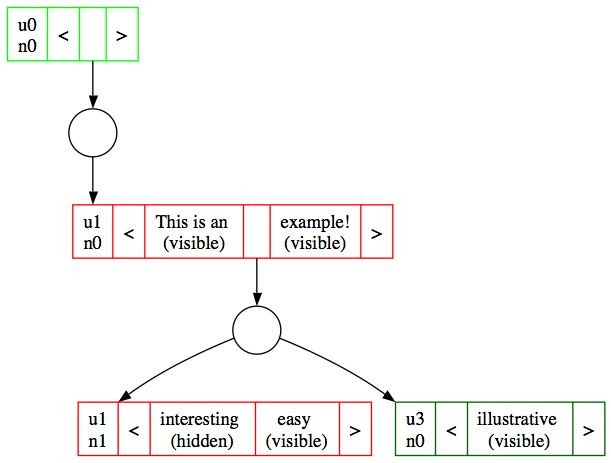
\includegraphics[width=3in]{tree14d.jpg}

\caption{An additional option if the insert was by user 1.
Observe that the text ``easy'' appears with the label ``visible''
in the node $u1/n1$ following the pre-existing hidden text
``interesting'' This is a valid edit operation only if the user
that created the insertion operation is the owner of the node
being extended. In this case, both are $u1$. \label{fig:tree14d}}

\vspace{\baselineskip}%
  \hspace{\fill}\rule{\linewidth}{.7pt}\hspace{\fill}%
\vspace{\baselineskip}%
\end{figure}

Note that we could not insert node $X$ directly before the $<^1_1$ marker
as that would violate the property of edit-trees that all children of a
node attached at the same point must be ordered by their userid and there
must be at most one node for each user. In this case, user 1 would have two
nodes inserted at position 11 of $u1/n0$ which is not allowed.

\subsection{General features revealed by the example}
This extended example demonstrates the fundamental ideas behind the MSET
approach. Each user $u_i$ represents the shared document as an edit-tree $T_i$
which has three different views: the standard view  which
is the string of visible characters in $T_i$, a revision string view which shows both visible and hidden characters (possibly with strike-through font) and an edit-string view which contains the hidden characters as well as the
start and end markers for the nodes. The user can insert and delete anywhere
in the standard view, but can only mark characters as "hidden" in the
edit-string view and can only insert at selected places in the edit-string
view. The string operations are converted to edit-tree operations which are
broadcast to all of the peers in the collaborative editing group. Those users
apply the remote operations they receive in any order they choose, provided only
that they wait for the target node of an operation to be created before the'
operation is applied.

We will describe the algorithm in more detail below and we will show that it
can be implemented in such a way that each local and remote single character 
edit operation
can be performed in time $O(\log(N))$ where $N$ is the size of the edit-string.



\section{The unoptimized distributed model for edit trees}
\label{sec:edittrees}
% Here we describe the model at the level of nodes without worrying about an efficient
% implementation. We can describe the late joining protocol and the central server vs
% distributed server model.

As mentioned in the introduction the MSET model is based on the notion that 
each user maintains an edit tree as the underlying model of the textarea in
which they are editing. In this section, we describe an algorithm for 
collaboratively editing the edit-trees directly. In a later section we will show 
how to implement these algorithms
efficiently. In this section, we assume that the users are only interested in editing
the trees directly. This algorithm is essentially the same as the TreeDoc data type of Preguica, et. al. The main innovation of this paper is that it shows how to use this tree structured data type to implement an optimally efficient text editor.

\subsection{Definition of an edit-tree}
We make the following assumptions about the structure of the edit-trees:
\begin{itemize}
\item Each user has a unique ID from some totally ordered set $U$ of userids 
and the nodes of the edit-tree 
are labelled with the userid and an integer which uniquely identifies
that node among all created by that user.
\item Each node contains a sequence of one or more characters.
\item Each character has a boolean visibility property which is set
to false when the character is "deleted". 
\item The nodes can have children nodes.
Each such child is attached at a particular position in the string.
\item Multiple nodes can attach to the same position, but no two nodes that are owned by the 
same user can be attached at the same position. The nodes that are attached at
a given position are ordered by userid. 
\item The root of the tree is owned by the
superuser "u0". This user does not own any other nodes and does not insert any
text into the root node. 
\end{itemize}

\subsection{Valid edit operations on an edit-tree}
We place restrictions on the type of edits that can be performed
on an edit tree.  We will indicate nodes 
of the edit-tree being edited by
the notation $u/n$ where $u$ is the user who created the node and $n$ is an
integer uniquely identifying this node among all nodes created by the user.

There are three operations a user $u$ can perform on a node and the operations
that can be performed depend on the user. To simplify the presentation, we only consider operations that handle a single character at a time.

Let $v/m$ denote the $m$th node created by user $v$.
User $v$ will be able to append characters to the end of $v/m$, so 
we will sometimes futher indicate that node by $(v/m:p)$
where $p>0$ is the number of characters in $v/m$. This allows us to
distinguish between different versions of a single node.

Let $u$ be the user performing one of the following tree tree edit operations
on the target node {\tt v/m:p} to create a new node {\tt u/n:q}.
\begin{itemize}
\item ${\tt treeextend}(v/m:p,c)\;\;\text{if u=v}$ \newline
First, user $u$ can extend the text in the node $v/m$
provided it is the owner (that is $v=u$). It extends the node by appending
some character $c$ to the location $p$ at the end of the node,
Note however, that users can not modify
the text in any node that they do not own and can not change any of the text
once it has been put into the node.
\item ${\tt treeinsert}(v/m:p,q,u/n:1,c) \;\; \text{if $q\le p$}$
\newline
Second, user $u$ can insert a new node $u/n$ containing a character $c$
at any position $q\le p$ of the node, 
$v/m$ provided
they have not already inserted a node there. If one or more nodes have already been inserted there, then they must be arranged in order of the userid and the new node is inserted into this sorted sequence by userid.
\item ${\tt treehide}(v/m:p,q)  \;\; \text{if $q < p$}$\newline
Third, user $u$ can set the visibility of a character at position $q < p$
in  $v/m:p$ to false.
When characters are initially added to a node they have visibilty true, but once
set to false, the visibilty must remain false. 
\end{itemize}
For all of these operations, we say that the node $(v/m:p)$ is the target of the edit operation and the node that is created, either $(v/m:p+1)$ for an extension or $(u/n:1)$ for a new node, is the result.  

We use these definitions to define a partial order on edit operations $\tau\prec\tau'$ where $\tau$ directly precedes $\tau'$ if the result of $\tau$ is the target of $\tau'$, and we let $\prec$ be the transitive closure of that relation.  Then $\prec$ is a partial order on the set of all possible edit operations on a tree. We say that two operations $\tau$ and $\tau'$ are independent if neither precedes the other, that is 
\[
\left (\tau\not\prec\tau'\right ) \wedge  \left ( \tau'\not\prec\tau \right )
\]
Observe that operations performed simultaneously by two clients on their own local edit trees are clearly independent from each other.

Given these definitions and rules we see that a group of distributed users can easily edit a 
shared tree by keeping their own representation of the tree and broadcasting
their edits to their peers. Observe that these edit operations commute in
the following sense. The only place where two users could have a editing
conflict is when they both want to insert a string of characters at a particular
position $q$ in some node $v/m:p$, but in this case their insertions are always
ordered by userid and this resolves the conflict. No matter which order the
operations are applied the same tree results. This is phrased more formally
in the following lemma:

\begin{lemma}
Let $T=T_0$ be any edit-tree and let $\tau_0,\tau_2,\ldots,\tau_{n-1}$
be a sequence of valid edit operations on $T$ as described above.
This yields a sequence of edit trees $T_0,\ldots,T_n$. Let 
$\tau'_0,\ldots,\tau'_{n-1}$ be any reordering of this sequence of operations
which is topologically sorted with respect to $\prec$, that is
with the property that if $i<j$ then either $\tau'_i\prec\tau'_j$ or
$\tau'_i$ and $\tau'_j$ are independent. Let $S_0=T_0$ and $S_{i+1} = \tau'_i(S_i)$.
Under these assumptions, the corresponding sequence of trees
$S_1,\ldots,S_n$ is well-defined and $S_n=T_n$.
\end{lemma}

\begin{proof}
First, the sequence $S_{i}=\tau'_i(S_{i-1})$ is well-defined because we have
stipulated that the target of each $\tau'_i$ must exist in $S_{i-1}$ so the
operator can be applied. To see that the two resulting trees are equivalent
we simply observe that the extend operations for a node $v/m:p$ must appear
in the same order in the $\tau'_i$ as the $\tau_i$ and since they effect only
the node $v/m$ the node $v/m$ will contain the same string in both $S_n$ and $T_n$.
The insert operations for a given node $v/m$ on the other hand can appear
in any order and their effect will be to add children to positions $q$
of the final node. When multiple insertions attach to the same position, they
will be ordered by user id. Since they are inserted into an ordered list,
the order in which they are inserted doesn't matter.
\end{proof}

\subsection{Distributed editing of edit trees}
In the previous subsection we showed that any valid ordering for a sequence
of tree edit operations will yield the same final result. We can use that
observation to define a distributed algorithm which converges provided only
that a fair network property is assumed.

The model is that we will have a set $G$ of clients $C_1,\ldots,C_n$
all starting with the empty tree. Each client $C_i$ has a unique userid $u_i$,
a local copy $T_i$ of the shared edit tree,
a list $Q_i$ of edit operations that other users have applied but which it
has not yet processed, and
and a map $H_i$ from nodeids $v/m$ to nodes of the edit tree or to sets of tree-edit operations using a union type. If the tree $T_i$ contains a node $A$ with nodeid $v/m:p$ then $H_i(v/m:p)=A$, otherwise $H_i(v/m:p)$ is a list $S$ of tree-edit operations taken from $Q_i$ whose target is $v/m:p$.

We assume that the clients observe the following protocol. 
In particular user $u_i$ can do the following:
\begin{itemize}
\item Perform a valid operation $\tau$ on their local copy of the tree to
produce a new (or extended) node $n$ with nodeid $u/n:q$,
after which they set $H_i(u/n:q)$ to $n$ and they also add $\tau$ to $Q_j$ for
all $j\ne i$.
\item Take an operation $\tau$ from $Q_i$. If the target of $\tau$ is
in $T_i$ then $\tau$ is applied to the tree to produce a node $v/m:p$
and the tree-edit operations in $H_i(v/m:p)$, if any, are inserted back into $Q_i$
 and $H_i(v/m:p)$ is set to $n$.
\end{itemize}
Note, this model can easily be extended to allow for late joiners by having users
maintain a history list $Q'_i$ of all operations they have applied to their tree.  Any user $k$ who joins the group notifies all users it has joined and waits for confirmation from all users. Once this is obtained, it 
requests some client $C_j$ to forward its current history list $Q'_k$ and its current queue, 
$Q_k$ into its own edit queue $Q_i$.
This can be an incremental copy at user $j$'s leisure depending
on the workload.  This may require user $k$ to check each new operation
it receives to make sure that it has not already been received and processed,
but this is not too expensive.

\begin{lemma}
Let $G$ denote a collaborative editing session as described
above and assume that all clients $C_1,\ldots,C_n$ follow the protocol above
for a certain period of time and then stop. Once all queues $Q_i$ have been
emptied and all operations processed, all users will have the same edit
trees, that is if $T_i$ is the final edit tree of $C_i$, then $T_1=T_2=\ldots=T_n$.
\end{lemma}

\begin{proof}
This follows easily from the previous lemma where we let $\tau_1,\ldots,\tau_m$
denote the sequence of operations performed by user $1$ and let 
$\sigma_1,\ldots,\sigma_m$ denote the operations performed by user $i$. Then
these are clearly valid rearrangements of each other and by the previous
lemma the resulting trees are the same.
\end{proof}

\section{From edit-trees to an optimally efficient collaborative editor}
\label{sec:proof}
In this section we will define the MSET data type $M$ which simultaneously maintains
four views of an editing session
\begin{itemize}
\item $M.S$ - the standard string view of a text-editing session, a sequence of characters from a character set $\Sigma$
\item $M.R$ - a revisions view which is a sequence of characters which each have a visibility attribute (visible or hidden), this is similar to the tracking-changes view of many modern text editors
\item $M.E$ - an edit-string view which is a sequence of attributed characters and marker symbols (start markers $<^u_n$ and end markers $>^u_n$)
\item $M.T$ - an edit tree
\end{itemize}
The three string views are all views of the edit tree $M.T$ obtained by traversing the tree in infix order and recording the characters and or symbols of the specified type.

Our approach will be demonstrate that insertions and deletions on $M.S$ can be
transformed efficiently (in time $O(\log(N))$ where $N$ is the size of $M.T$) into
tree-edit operations on $M.T$.  We will also show that the three tree-edit operations
on $M.T$ can be performed in time $O(\log(N))$ and that for each tree-edit operation $\tau$ we can calculate the corresponding string edit operations on $M.S$, $M.R$, and $M.E$ in time $O(\log(N))$.  If we assume that we have a system which will maintain the string views of $M.S$, $M.R$, and $M.E$ then this approach allows us to accept string-edit operations on $M.S$ from the user, use them to construct a corresponding tree-edit operation $\tau$ and then broadcast that $\tau$ to all other users.  Moreover, for each tree-edit operation $\tau$ generated locally or received from a remote user, the corresponding string-edit operations $\sigma_S, \sigma_R, \sigma_E$ can be efficiently generated and sent to the systems which are maintaining those views.

In this section, we define the MSET data type and prove that its operations can be performed in time $O(\log(N))$ where $N$ is the size of $M.T$.

The data type $M$ is created in constant time by a constructir $MSET.new(u)$ that creates an empty tree $M.T$ and empty strings $M.S, M.R, M.E$ for the user $u$.

The data type $M$ allows the following operations:
\begin{itemize}
\item $M.treeextend(v/m:p,c)$ - lookup the node with nodeid v/n:p and extend it by adding the character $c$ at position $p$, update the lists $M.S$, $M.R$, and $M.E$ as well.
\item $M.treehide(v/m:p,q)$ - set the visibility to false for the element at position $q$ of the node with id $v/m:p$
\item $M.treeinsert(v/m:p,q,u/n,c)$ - create a new node with id $u/n:1$ containing the single visible character $c$ and insert that new node at offset $q$ in the node with id $v/m:p$.
\item $M.converttotreeop(\sigma)$- returns a tree-edit operation $\tau$ on $M.T$ that corresponds to the string edit operation $\sigma$ on $M.S$
\end{itemize}
We will provide algorithms for these operations and prove that their complexity is $O(\log(N))$.
\subsection{implementation of characters and markers}
We assume all visible characters come from an alphabet $\Sigma$
and we expand that to an alphabet $\Sigma^*$ which also includes all start and end markers.

%The elements in the lists and the tree will be represented by a tuple that contains
% links to the nodes and also links to an indexing object $M.I$ which will allow one
% to rapidly calculate the position of the element in the lists (i.e. the number of
% elements of type $S$, $R$, or $E$ to the left of the element) and also allows us to
% rapidly find the $k$th element of each of the three lists.

We represent the elements of these strings by tuple containing
\begin{itemize}
\item {\tt symbol} - a character or start marker or end marker 
\item {\tt visible} - a boolean used to distinguish visible from hidden characters
\item {\tt marker} - a boolean used to distinguing markers from non-markers
\item {\tt node} - a link to the node of the edit tree containing this element
\item {\tt nodeid} - a convenience field giving the id $v/m:p$ of the node
\item {\tt offset} - the offset of the element in the node, which is either a non-negative integer or is {\tt start} or {\tt end} for the markers.
\item {\tt indexTree} - a link to the index tree node corresponding to this element
\end{itemize}

\subsection{Implementation of the lists $M.S$, $M.R$, and $M.E$}
The three lists will be represented by doubly linked lists together with an index
tree that provides $O(\log(N))$ access to the elements by their offset in the three lists. 

The index tree $M.I$ can be implemented as a balanced binary tree whose leaves are the elements in $M.T$ and which stores at each internal node, a triple containing the number of elements of type $S,R,E$ in the subtree below that node,
see 
Figure \ref{fig:indextree} for an example. 

\begin{figure}[h]
\centering
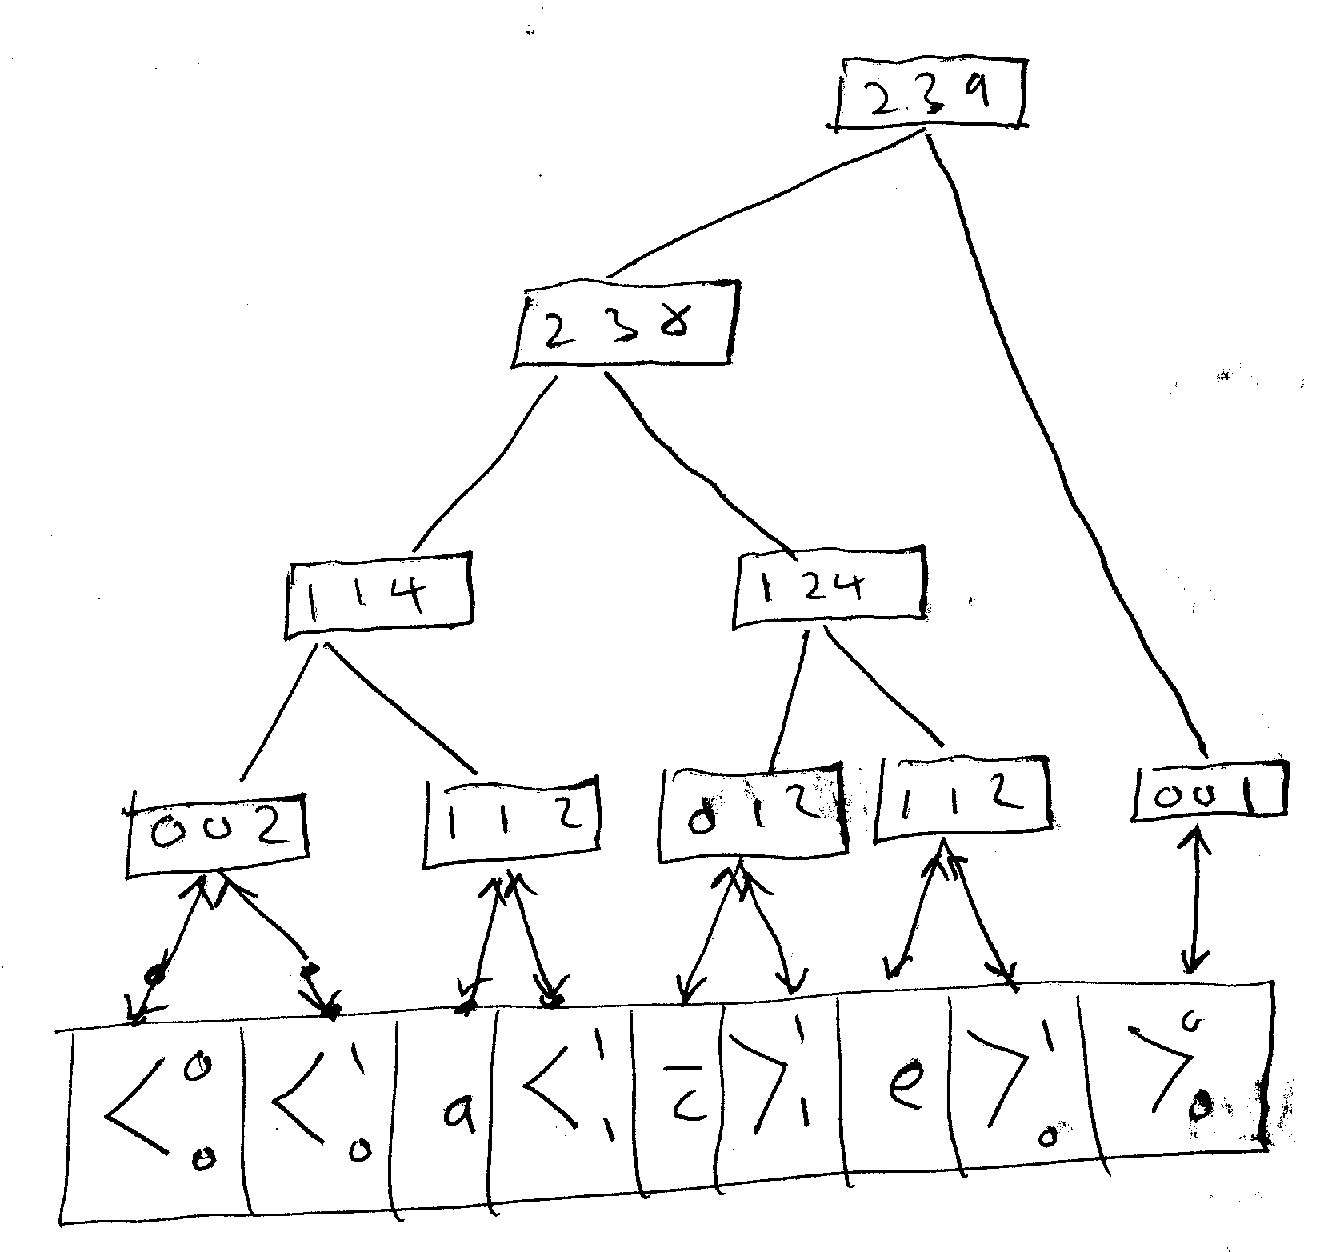
\includegraphics[width=3.0in]{MSETfig002.jpg}
\caption{Index tree for the three lists. \label{fig:indextree}"}
\end{figure}


Clearly such a structure can support insertion of elements in time $O(\log(N))$ by inserting and rebalancing (e.g. with red/black trees) and then updating the element count triples in the modified nodes. This structure allows us to implement the following  operations so they can be computed in time $O(\log(N))$ where we assume we have already calculated the node and offset for $e$ in $M.T$
\begin{itemize}
\item {\tt M.insertBefore(e,f)} - insert element $e$ before element $f$ in $M.E$ and reflect those changes in $M.R$ (resp. $M.S$) as well so that they remain the subsequence of $M.E$ consisting of non-marker (resp. visible) elements.
\item {\tt M.insertAfter(e,f)} - similar to the above, but insert $e$ after $f$
\item {\tt M.insertAtStart(e)} - insert $e$ at the beginning of $M.E$.
\item {\tt M.hide(e)} - this sets the visibility of $e$ to $false$ and removes $e$ from $M.S$, updating the indexTree $M.I$ in the process.
\end{itemize}



\subsection{Implementation of the tree $M.T$}
The edit tree will be implemented as a rooted set of linked nodes as shown in Fig. \ref{fig:MSETtree}. 
\begin{figure}[h]
\centering
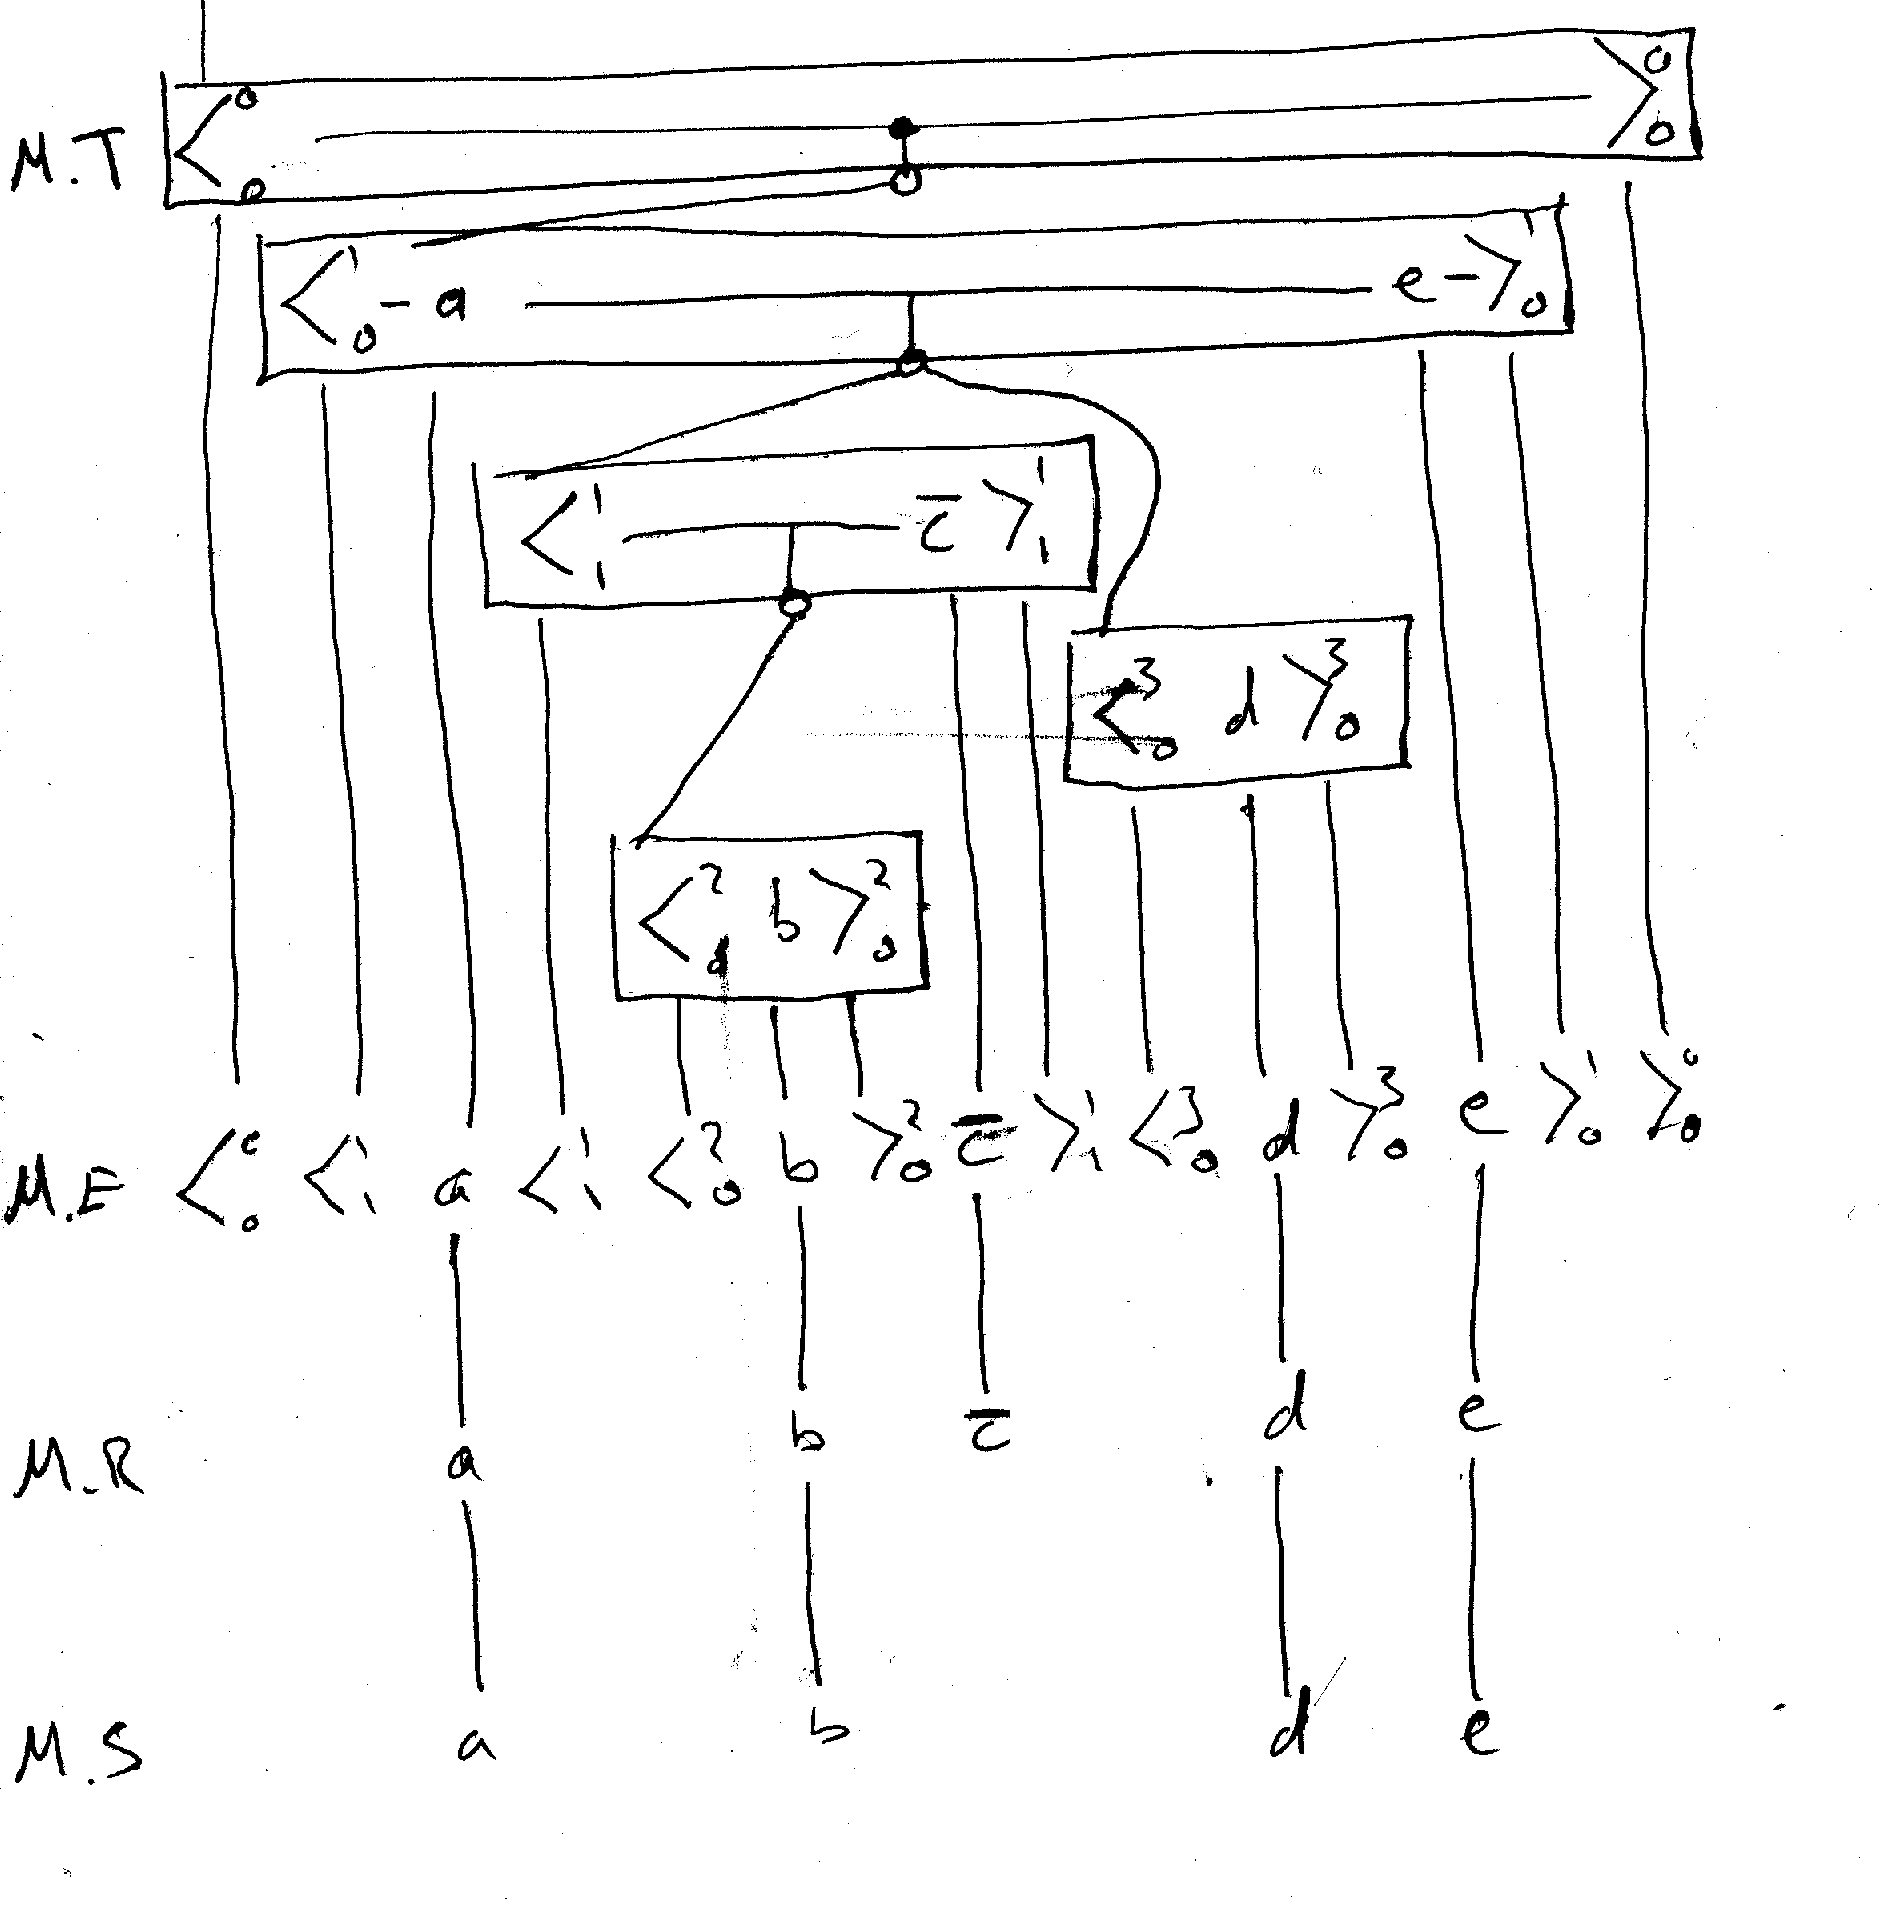
\includegraphics[width=3.0in]{MSETfig001.jpg}
\caption{MSET tree and lists\label{fig:MSETtree}"}
\end{figure}
The nodes contain a sequence of elements as well as the links to children nodes
Each node has the following fields:
\begin{itemize}
\item {\tt userid} - the unique id for the user who created this node
\item {\tt count} - the number of nodes created by that user before this one
\item {\tt elt[]} - an array list of elements
\item {\tt insertionSet[]} - an array list of insertion sets providing access to the children nodes inserted at each position in the node
\end{itemize}
Each {\tt insertionSet} maintains a sequence of nodes, ordered by userid where
each element can be accessed in $O(\log(N))$ time (actually $O(\log(U))$ time where $U$ is the number of users active in creating $M.T$ but that is less than or equal to the number of nodes in $M.T$).




\subsection{Efficient implementation of $M.converttotreeop(\sigma)$}
This function takes a string operation $\sigma$ on $M.S$ and converts it into
an equivalent tree operation 
$\tau$ on $M.T$ such that
$\Gamma(\tau(M.T)) = \sigma(\Gamma(M.T))$, where $\Gamma(T)=S$ is the standard string representation of the tree $T$; and likewise for $M.R$ and $M.E$.

There are two possibilities for $\sigma$, either it is an insertion of a character $\alpha$ at offset $k$ in $M.S$ or it is the deletion of the character $\alpha$ at position $k$ in $M.S$.  

 {{\tt delete($k$)}} 
Lets handle the deletion case first as it is easiest. The first step is to lookup the element $e$ at position $k$ in $M.S$. This can be done in time $O(\log(N))$.
We can then use $e$ to lookup the node $n$ and offset $q$ of $e$ in that node.
This takes time $O(1)$, as the node and offset are fields of $e$. Finally, we lookup the
nodeid $v/m$ and length $p$ of $n$ and generate the operation $treehide(v/m:p,q)$. This operation takes time $O(\log(N))$. In pseudocode, we have
\begin{verbatim}
delete(k)
  e = M.I.lookupS(k);
  v/m:p = e.nodeid;  q = e.offset
  return treehide(v/m:p,q)
\end{verbatim}

Next lets handle the case where $\sigma$ is the insertion of the character $c$
at offset $k$ of the string $M.S$.  There are five cases to consider:

\begin{figure}[h]
\centering
\includegraphics[width=4.0in]{insertAtFront002.jpg}
\caption{Inserting a character at the beginning and end of $M.S$ \label{fig:frontinsert}"}
\end{figure}

\subsubsection{Case 1: inserting at the beginning of a string: $k=0$}
In this case, we are to insert $c$ at the beginning of the string.
The first step is to look up the first element $e$ of $M.R$ in time $O(\log(N))$.
This is the first non-marker element in $M.T$. Using $e$ we lookup the
nodeit $v/m:p$ of the node containing $e$ and we observe that $e$ must be at position 0 in this node (as it is the first non-marker element in $M.E$. Therefore
we generate the tree operation $treeinsert(v/m/p,0,u/n,c)$. This takes total time $O(\log(N))$.
\begin{verbatim}
insertcase1(k,c)
  e = M.I.lookupR(0);  n = e.node; v/m:p = e.nodeID
  return treeinsert(v/m:p,0,u/n,c)
\end{verbatim}



\subsubsection{Case 2: inserting at the end of a string}
This case is similar. We start by looking up the last element $e$ in the revisions view $M.R$ which is also the last non-marker element in $M.E$. This takes time $O(\log(N))$, we can also look up the nodeid $v/m:p$ of the node in time $O(1)$.  There are
two cases, if $u=v$ then we can generate a tree extend operation
$treeextend(v/m:p,c)$ and otherwise we generate a insert operation
$treeinsert(v/m:p,p,u/n,c)$.
\begin{verbatim}
insertcase2(k,c)
  e = M.I.lookupR(R.length);  n = e.node; v/m:p = e.nodeID
  if u==v then return treeextend(v/m:p,c)
              else  return treeinsert(v/m:p,p,u/n,c)
\end{verbatim}

\begin{figure}[h]
\centering
\includegraphics[width=4.0in]{insertMiddle001.jpg}
\caption{Cases 3a,3b: Inserting between two characters in $M.S$ \label{fig:midinsert}"}
\end{figure}

\begin{figure}[h]
\centering
\includegraphics[width=2.0in]{insertMiddle002.jpg}
\caption{Case 3c: inserting between two characters of $M.S$ \label{fig:frontinsert}"}
\end{figure}

\subsubsection{Case 3: inserting in the middle of the string}
in this case we can lookup the elements $e$ and $f$ on either side of the insertion point $k$ in $M.S$. This takes time $O(\log(N))$.  We can look up the offsets $k_1$ of $e$ in $M.E$ and $k_2$ of $f$ in $M.E$ and look at the elements between $e$ and $f$ in $M.E$. There are three subcases to consider here depending on the type of the element $g$ that follows $e$ in $M.E$.

\subsubsection{Case 3a: $g$ is a non-marker element}
In this case, $g$ is either $f$ or a hidden character, but in any case, we can insert $\alpha$ between $e$ and $g$. So in time $O(1)$ we lookup the nodeid $v/m$ and
offset $q$ of $g$ and generate the tree edit operation 
$treeinsert(v/m:p,q,u/n,c)$

\subsubsection{Case 3b: $g$ is an end marker}
In this case, we look up the node id $v/m$ of $e$ as before and if $u=v$
then we can extend the node with $treeextend(v/m:p,c)$ whereas if $u\ne v$
then we use a standard insertion $treeinsert(v/m:p,q,u/n,c)$.


\subsubsection{Case 3c: $g$ is a start marker}
in this case, all of the nodes between $e$ and $f$ must be start markers,
so we can insert $\alpha$ directly before $f$.  Look up the nodeid $v/m:p$ of $f$
in $O(1)$ time and generate $treeinsert(v/m:p,0,u/n,\alpha)$

\begin{verbatim}
insertcase3(k,c)
  e = M.I.lookupS(k-1); f = M.I.lookupS(k);
  v/m:p = e.nodeid; 
  g = e.nextE /* get element after e in M.E */
  if not g.isMarker
    treeinsert(g.nodeID,g.offset,u/n:1,c)
  else if g.isStartMarker
    treeinsert(f.nodeID,0,u/n,c);
  else if g.isEndMarker & u==v
    treeextend(v/m:p,c)
  else
    treeinsert(v/m:p,p,u/n,c)
\end{verbatim}
We have consider all of the possible cases and hence this demonstrates that 
$M.converttotreeop(\sigma)$ can be implemented with complexity $O(\log(N))$.




\subsection{implementing $treehide(v/m:p,q)$}
The first step is to lookup, in time $O(\log(N))$ the node $n$ with id $v/m:p$
and to then look up the element $e$ at offset $q$ in time $O(1)$. 
To hide $e$ we simply set the visible value to $false$.

Once we've found the element $e$ to be hidden, we can
calculate the position $k_S$ of the element in $M.S$ in time $O(\log(N))$
and generate the string op $delete(k_S)$. The same process can be applied to
$M.R$ and $M.E$ to generate $delete(k_R)$ and $delete(k_E)$, which should
change the view for the character to indicate it has been "deleted".

\begin{verbatim}
treehide(v/m:p,q)
  n = M.lookupNode(v/m:p);
  e = n.elt[q]
  M.I.hide(e)
\end{verbatim}


\subsection{applying $treeextend(v/m:p,c)$ on $M.T$}
Again, we first lookup the node $n$ with id $v/m:p$ in time $O(\log(N))$ and then lookup the 
end marker element $f$ of $n$. We can then create a new element $e$
using $c$ and the node id $v/m:p$. We can then insert $e$ into
$M.E$ by inserting it before the end marker $f$ of $n$ and then adjust 
the indexing trees for $M.S$, $M.R$, and $M.E$.

Using this node $n$, we can calculate the number
of elements $(k_s,k_r,k_e$ of each type (visible, non-maker, any) that appear before $e$ in
the three lists (in time $O(\log(N))$ and generate the string ops $stringinsert(k_X,\alpha)$ for $X \in \{s,r,e\}$ to update the string views.

\begin{verbatim}
treeextend(v/m:p,c)
  n = M.lookupNode(v/m:p);
  f = n.endmarker
  e = Element.new(c,n)
  M.I.insertBefore(e,f)
\end{verbatim}

\subsection{applying $treeinsert(v/m:p,q,u/n,c)$ to $M.T$}
In this case, we need to lookup the target node $A = M.lookupNode(v/m:p)$ create a new node $B$ containing a single element
$e_2$ which contains the visible character $c$. We also need to create elements $e_1$ and $e_3$ representing the start and end markers for node $B$, respectively.
Then we need to insert $B$
into the insertion set $S=A.iset[q]$ of the target node $A$ in time $O(\log(N))$ 
and to complete this operation we only need to insert the elements $e_1,e_2,e_3$ into the correct place in $M.E$

\begin{figure}[h]
\centering
\includegraphics[width=1.0in]{insertTree001.jpg}
\caption{Inserting into $M.T$ when $S$ is empty \label{fig:emptyS}"}
\end{figure}

\begin{figure}[h]
\centering
\includegraphics[width=2.0in]{insertTree002.jpg}
\caption{Inserting into $M.T$ when $S$ is non-empty \label{fig:nonemptyS}"}
\end{figure}

Lets first consider the case where $S$ is empty, that is, nothing has yet been inserted. 
 Figure \ref{fig:emptyS} illustrates this situation. We are inserting a new node containing the elements $<^u_n c >^u_n$ between two elements $c_1$ and $c_2$ of node $A$.
In this case, the three elements $e_1,e_2,e_3$ will appear directly after the start marker $c_1$,
so we invoke $M.E.insertAfter(e_1e_2e_3,c_1)$.  
Note that if $q=0$, then $c_1$ is the start marker, $A.start$, otherwise $c_1=A.elt[q-1]$.
This can be performed in $O(\log(N))$ time.

If $S$ is not empty, then when we insert $B$ into it, it either appears as the first node in the insertion set, or the last node, or it appears between two nodes $C$ and $D$. In all of these cases, $B$ is either immediately before or immediately after another node $C$. Figure \ref{fig:nonemptyS} shows this situation.

If $B$ is before a node $C$, then we insert $e$ before the start marker of $C$ with
$M.E.insertBefore(e,C.start)$. If $B$ appears immediately after a node $C$ in $S$,
then we insert $e$ after the end marker of $C$ with
$M.E.insertAfter(e,C.end)$.


\subsection{Main theorem}
We have therefore proved 

\begin{theorem}
The implemenation of the MSET data type described above requires at most
$O(\log(N))$ time to process any of the local string operations, that is,
 insert or deleting a character at offset $k$, and
any of the three edit-tree operations (treeextend, treeinsert, treehide), where $N$ is the size of the edit-tree before the operation is performed.
\end{theorem}

\section{MSET-based Collaborative Editing}
\label{sec:collabed}
In this section we describe how to use the MSET data type to implement a convergent collaborative editing system among a group $U = \{u_1,\ldots,u_r\}$ of users.

In the simplest model, all users start off with an empty MSET. We assume that the users can send messages to all of the peers using a broadcast command. 

Each user performs local edits on his or her string. These string edit operations are converted into tree edit operations and are applied to the user's tree as well as being broadcast to all of the peers.  Users collect tree edit operations from their peers in a queue $Q$. When they process a tree edit operation $\tau$ from $Q$, they first check to see if its target node $A$ is in their tree $M.E$.  If not, then the operation is added to a set $M.W(A)$ of operations waiting for target node $A$.  If $A$ is in the tree, then $\tau$ is applied and it produces a result node $B$. The elements in $M.W(B)$ that were waiting for $B$ to be created are now added to the front of $Q$.

We call such a system the Basic MSET Collaborative Editing session. In the previous section we proved that each editing operation requires time at most $O(\log(N))$ to process by both the user orginating the edit operation and all of the peers processing it on their own trees.  Since insertion into a list requires time $O(\log(N))$ we see that, in terms of the amount of time to process each edit operations, this is an optimally efficient algorithm.

\section{Potential Pitfalls with MSET Collaborative Editing}
\label{sec:pitfalls}

\subsection{Editing overload}
If too many users are editing a document at the same time, it can result in such a high load of edit operations that the users will not be able to keep up.

For example, suppose that there are $R$ users each generating $G/\log(N)$ operations per second (where the logarithmic term accounts for the slowdown that occurs as the tree gets larger). Further, suppose that each user can process $P/\log(N)$ operations per second. Then, the rate at which edit operations are generated in the collaborative editing session is $R*G/\log(N)$ and users will
not be able to keep up if this exceeds their processing rate, i.e. if $P<R*G$.
Thus, if we assume that $P$ and $G$ are some standard rates for users on
typical hardware, this puts a limit on the number of users the system can support based on the average values of $P$ and $G$, viz. $R < P/G$.

This can be solved by using faster hardware (i.e. increase $P$) but is a fundamental
problem with scalability in collaborative editors.  There is also the cognitive overload problem of trying to imagine editing a document with a very large
number (e.g. a million) simultaneous co-editors.   

\subsection{Bottlenecks caused by a connection slowdown}
Another class of problem arises if one of the peer-to-peer connections, say from $u_1$ to $u_2$ becomes too slow. This can create a bottleneck for $u_2$ which
can effectively freeze all outside editing operations. 
Suppose that $u_1$ performs 
an editing operation $\tau$ that creates a node $A$ and it sends that operation rapidly to
all users $u_3,\ldots,u_n$ but there is a very long delay before it can send $\tau$ to $u_2$.  In the meantime, assume that
all of the other users $u_3,\ldots,u_n$ are building upon
this target node $A$. The user $u_2$ will receive and need to enqueue all of the operations of users $u_3,\ldots, u_n$ until it receives this "bottleneck" operation $\tau$. When $\tau$ finally is
received and node $A$ is created, all of the operations waiting on $A$ and its descendants must be processed.  It may take a substantial amount of time for $u_2$ to process the backlog
even though each individual operation requires only $O(\log(N))$ steps.  

Such a situation can be minimized by allowing users to send "pull" requests to peers for edit operations that create a particular target, but this can increase the network traffic and slow down the system as well.


\section{Practical Implementations}
\label{sec:implementation}
We have implemented a variant of the MSET data type and used it to create plugins for standard IDEs (jEdit, Eclipse, Netbeans) and our own editors \cite{granville_collabed:_2009}.  This variant introduced several
practical enhancements to improve performance (though not asympotically)
and to improve the user experience.  In this section, we briefly describe these
enhancements.

\subsection{Subnodes}
One problem with the MSET implementation described above is that there is a high overhead required for each character in the edit string. This can create a 10-50 fold increase in space and also a corresponding slowdown in execution time. For example, just loading in a single 100K text file will require three doubly-linked lists with indexing for each character in the text file.

We tackled this problem by representing the lists $M.S$, $M.R$, and $M.E$ as lists of subnodes rather lists of single characters, where a subnode is a sequence of continguous characters in a node which is not interrupted by an non-null insertion set and in which all of the characters have the same visibility (i.e. the are either all visible or all hidden).  When a textfile with $N$ characters is loaded into an MSET structure the
result is a single node and the lists $M.S$, $M.R$ each contain a single subnode which is just a pointer to the main node with indices for the start (0) and end ($N$) indices. The list $M.E$ has three subnodes as we represent the start and end markers as their own separate subnodes. 

The use of subnodes introduces the extra complication of having to manage the list of subnodes with in a node (and to split a subnode if there is an insertion within it or if one of the elements inside is set to hidden from visible).  The advantage of this approach is that copy and paste operations can be implemented as a single edit operation that creates a new node containing an entire string, not just a character.
For example, when a large string is copied and pasted, the modified MSET algorithm tree will add a single node
containing one large string to the tree, and the corresponding subnode will be
inserted into the lists. Finally, the user will send out one edit operation containing that string to all peers.

Likewise, deletion can be implemented by having a single visibility flag on an entire subnode so that cutting a large section of text can be done by setting the subnodes' visibility flags to false rather than setting each individual element's flag to false. In general, deleting a region may cause many subnodes to be marked as hidden.

\subsection{Attributes}
Building on the subnode model, we extended MSET to allow for each subnode to contain a set of attributes (e.g. font, style, color, etc.). To handle the inevitable conflicts, we used a protocol where each attribute had an associated version number and associated user id of the user who set that attribute's value.  When there is a conflict, the edit operation with the highest version number wins, and if there is a tie, then the one with the highest user id wins. If attribute version numbers are
represented as fixed size fields, then the number of times an attribute can be changed is limited.  If the version number is a "bignum" of unbounded size, then there is no maximum number of attributes but the space (and time) complexity of the system increases logarithmically in the version number.

\subsection{Manual Queueing of Incoming and/or Outgoing Edit Operations}
We have found it useful to maintain queues of incoming and outgoing edit operations
and to allow the user to temporarily stop processing incoming edit operations (and hence allowing the incoming queue to grow).  This is useful if the user wants to perform some edits without being distracted by other users, for example, applying an emacs style repeated command that will process every line of a file with some particular sequence of edit operations.  Likewise, users may sometimes want to stop sending their edits to other users temporarily (and thereby allowing the outgoing edit queue to grow).  This can happen if they want to create a section of the document entirely by themselves and don't want any other user to see it until it is in a more finished form.  The MSET data type makes it very easy to implement these queues with no additional penalty beyond the time delay it will take to process the edit operations later rather than immediately. It has also turned out to be a feature that users often employ.

\subsection{Color coding the view}
We have also found it useful to arrange the string view so that the last 10 characters inserted by a user are highlighted with a color unique to that user (and that the user can select themselves!)  In earlier work developing collaborative editors based on operational transformation we found that this use of color coding greatly helped enhance the awareness features of the editors, allowing users to have a good sense of what the other users were doing.

%\section{Future work}
%\label{future}
%Two topics that we have not discussed are the implementation of undo operations
%and the implementation of cut and paste operations.  Undo can be implemented fairly easily by performing a character insertion to undo a character deletion, and vice versa, but this does not revert the MSET to a previous state, rather it grows the state.  It might be possible to do better than this, at least in special cases. There are also interesting variations of undo in which a user could choose to undo just one other user's operations (typically her own, or the edits of a disruptive user).
%We have not studied these interesting issues with MSET.
%
%The implementaiton of cut and paste operations is subtle. For example, if another user performs a cut and paste on the code in which you are currently editing, the natural effect would be for you to continue editing the code but have it transferred to a different part of the document.  The current system, based on single character insertion and deletion operations, would simply steal all of the characters from around you and move them somewhere else. This is not very natural, but it seems to be quite difficult to implement a "natural" cut and paste algorithm for MSET Collaborative editors and this is an area that ought to be considered.



\bibliographystyle{abbrv}


\bibliography{collabed}

%\appendix
%\section{Proofs}
%I think we claimed that we would put some things in the appendix!
\end{document}


%%% Local Variables: 
%%% mode: latex
%%% TeX-master: t
%%% End: 
